\documentclass[tikz, border=4pt]{standalone}
\usepackage{tikz}
\usepackage{tikz-cd}
\begin{document}
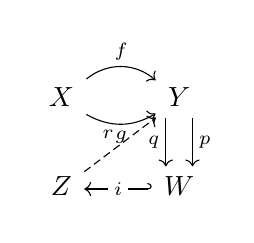
\begin{tikzpicture}[x=1cm, y=1cm]
  \node at (1.14,-1.08) {\pgfinterruptpicture%
  \begin{tikzcd}
    X \arrow[r, bend left=40, "f"] \arrow[r, bend right, "g"'] & Y \arrow[d, shift left=2, "p"] \arrow[d, shift right=2, "q"'] \\
    Z \arrow[ru, dashed, "r"] & W \arrow[l, hook', "i" description]
  \end{tikzcd}%
  \endpgfinterruptpicture};
\end{tikzpicture}
\end{document}
